\PassOptionsToPackage{unicode}{hyperref}
\documentclass[aspectratio=169, professionalfonts, 9pt, bibliography=totoc, xcolor={svgnames},
hyperref={colorlinks,citecolor=tudark,linkcolor=blue,urlcolor=DarkBlue}
]{beamer}

\usefonttheme[onlymath]{serif}
\usetheme[showtotalframes]{tudo}

\usepackage{polyglossia}
\setmainlanguage{german}
\usepackage[backend=biber]{biblatex}
\addbibresource{lit.bib}

% Mathematik
\usepackage{amsmath}
\usepackage{amssymb}
\usepackage{mathtools}
\usepackage{cancel}

\usepackage{hyperref}
\usepackage{bookmark}

\mode<presentation>

\usefonttheme{professionalfonts}
\usepackage{fontspec}
\usepackage[
    math-style=ISO,
    bold-style=ISO,
    nabla=upright,
    partial=upright,
    sans-style=italic,
]{unicode-math}
\setmathfont{Latin Modern Math}
\usepackage{listings}

% Paket float verbessern
\usepackage{scrhack}

% unverzichtbare Mathe-Befehle
\usepackage{amsmath}
% viele Mathe-Symbole
\usepackage{amssymb}
% Erweiterungen für amsmath
\usepackage{mathtools}

% Fonteinstellungen
\usepackage{fontspec}

% deutsche Spracheinstellungen
\usepackage{polyglossia}
\setmainlanguage{german}

% traditionelle Fonts für Mathematik
\setmathfont{Latin Modern Math}

\setmathfont{XITS Math}[range={scr, bfscr}]
\setmathfont{XITS Math}[range={cal, bfcal}, StylisticSet=1]

% Zahlen und Einheiten
\usepackage[
  locale=DE,                   % deutsche Einstellungen
  separate-uncertainty=true,   % immer Fehler mit \pm
  per-mode=symbol-or-fraction, % / in inline math, fraction in display math
]{siunitx}

% chemische Formeln
\usepackage[
  version=4,
  math-greek=default, % ┐ mit unicode-math zusammenarbeiten
  text-greek=default, % ┘
]{mhchem}

% richtige Anführungszeichen
\usepackage[autostyle]{csquotes}

% schöne Brüche im Text
\usepackage{xfrac}

% Standardplatzierung für Floats einstellen
\usepackage{float}
\floatplacement{figure}{htbp}
\floatplacement{table}{htbp}

% Floats innerhalb einer Section halten
\usepackage[
  section, % Floats innerhalb der Section halten
  below,   % unterhalb der Section aber auf der selben Seite ist ok
]{placeins}

% Seite drehen für breite Tabellen: landscape Umgebung
\usepackage{pdflscape}

% Captions schöner machen.
\usepackage[
  labelfont=bf,        % Tabelle x: Abbildung y: ist jetzt fett
  font=small,          % Schrift etwas kleiner als Dokument
  width=0.9\textwidth, % maximale Breite einer Caption schmaler
]{caption}
% subfigure, subtable, subref
\usepackage{subcaption}

% Grafiken können eingebunden werden
\usepackage{graphicx}
% größere Variation von Dateinamen möglich
\usepackage{grffile}

% schöne Tabellen
\usepackage{booktabs}

% Verbesserungen am Schriftbild
\usepackage{microtype}
\usepackage{tikz}
\usepackage[
  europeanresistors, % follow DIN
  americaninductors, % follow DIN
  siunitx,
]{circuitikz}

%Titel:
\title{Global Positioning System}
%Autor
\author[C.~Beckmann]{Christian Beckmann}
%Lehrstuhl/Fakultät
\institute[GPS]{Seminar - Physik des Segelns}
%Titelgrafik
\titlegraphic{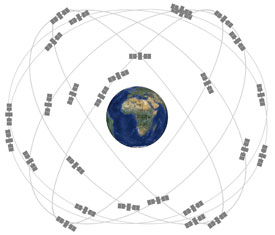
\includegraphics[width=0.3\textwidth]{images/constellation.jpg}}
\date{04. Dezember 2018}

\begin{document}
    \maketitle
    \begin{frame}
        \frametitle{Einführung}
        \tableofcontents%[pausesections]
    \end{frame}
    \section{Grundlagen}
    \begin{frame}
	       \frametitle{Grundlagen}
           \begin{block}{Betreiber}
               US-Regierung, Verteidigungsministerium
           \end{block}
           \begin{block}{Budget}
               2017: \$908,262 mil.\\
               2018: \$1,1 mrd
           \end{block}
           Bezahlt aus den Steuern der US-Bürger
           \cite{gpsgov}
       \end{frame}

       \begin{frame}{Historische Meilensteine}
           \begin{columns}
               \begin{column}{0.5\paperwidth}
                   \begin{itemize}
                       \item 1957: Sputnik
                       \item 1964: US-Marine, TRANSIT System
                       \begin{itemize}
                           \item Bill Guier (Mathematiker)
                           \item George Weiffenbach (Physiker)
                       \end{itemize}
                       \item Kalter Krieg
                   \end{itemize}
               \end{column}
               \begin{column}{0.5\paperwidth}
                   \begin{figure}
                       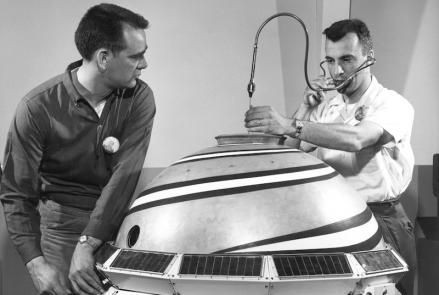
\includegraphics[width=0.4\paperwidth]{images/transit-satellite.jpg}
                       \caption{Tests am zweiten Transit Satelliten, \cite{TimeAndNavigation}}
                       \label{fig:transit}
                   \end{figure}
               \end{column}
           \end{columns}
       \end{frame}

       \section{Literatur}
       \begin{frame}{Literatur}
           \printbibliography
       \end{frame}
\end{document}
